\chapter{Analyse} % (fold)
\label{sec:analyse}
In diesem Kapitel sollen die in der Einleitung definierten Forschungsfragen untersucht werden. Um diese Fragen zu beantworten, wird eine Literaturanalyse durchgeführt, die bestehende Studien, Bücher und wissenschaftliche Artikel betrachtet. Ziel ist es, aus der vorhandenen Literatur systematisch Erkenntnisse abzuleiten, die die Performance der Ansätze in verschiedenen Szenarien beleuchten.

\section{FF-1: Wie unterscheiden sich GraphQL und REST hinsichtlich der Latenzzeit bei unterschiedlichen Anfragenkomplexitäten?} % (fold)
\label{sec:ff1}
Um zu untersuchen, wie GraphQL und REST sich im Bezug auf Latenz bei verschiedenen Anfragekomplexität auswirkt, muss man zunächst darauf eingehen, welche Faktoren oder Spezifikationen, die die APIS nutzen sich auf die Latenz auswirken.
Bei der Bereitstellung von Daten setzt REST auf HTTP-Endpunkte. Diese unterstützen nativ HTTP-Caching,  wodurch Ressourcen in einem Cache zwischengespeichert werden können um unnötige Datenübertragungen und Serveranfragen zu vermeiden und somit die Zugriffszeiten zu verringern.
Bei GraphQL wird dies nativ nicht unterstützt. Hierdurch können wiederkehrende Anfragen nicht gecached werden und müssen jeweils immer vom Server bearbeitet werden, wodurch eine höhere Zugriffszeit entsteht. \citep{graphqlreplacerest}

\noindent
REST fördert die Zerlegung von Systemen in eine Menge verknüpfter Ressourcen mit einem bestimmten Granularitätsgrad. Dies führt zu schwierigen Abwägungen zwischen Wiederverwendbarkeit und Leistung, die in der allgemeinen Software-Service-Architektur wohlbekannt sind. Weniger granulare und kohäsivere Services werden bevorzugt, da sie lose Kopplung und hohe Wiederverwendbarkeit fördern. Dies kann jedoch zu komplizierten Client-Server-Interaktionen führen, bei denen mehrere aufeinanderfolgende Anfragen notwendig sind, um die benötigten Daten aus dem Ressourcengraphen abzurufen,ein Phänomen, das als „Underfetching“ bekannt ist. Dieses Problem wird auch als n+1-Problem bezeichnet und tritt bei REST auf der Seite des Clients auf. Dieser muss dementsprechend weitere Anfragen schicken, bis die benötigte Antwortzeiten führen. \citep{graphqlhealth} \citep{migrategraphql}

\noindent
Bei GraphQL kann es ebenso zu einem n+1 Problem kommen. Hierbei tritt dieses jedoch nicht auf der Client Seite auf sondern direkt beim Server bei der Verarbeitung der Anfrage. Der GraphQL Server muss dann mehrere Anfragen an die Datenbank schicken, um die benötigten Daten zu erhalten, um sie dann an den Client auszuliefern.
\citep{graphqlsemantics}

\noindent
Hierfür bietet GraphQL einen sogenannten Dataloader, der die Anfragen, die zur Bearbeitung eines Requests benötigt werden bündelt und als eine einzelne, optimierte, Datenbankabfrage ausführt. \citep{nordstrom2022graphql}
\newline
\noindent
Zudem spielt bei der Latenz einer API die Anfragekomplexität eine entscheidende Bedeutung. In Abbildung 3.1 sind vergleichend die Ausführungszeiten von vier unterschiedlichen API-Abfragen, die sowohl mit REST als auch mit GraphQL durchgeführt wurden, zu sehen. Die Abfragen wurden auf den öffentlich zugänglichen GitHub REST- und GraphQL-APIs durchgeführt, da beide dieselben Ressourcen bereitstellen. Performance wird hierbei in Millisekunden gemessen und gibt Aufschluss darüber, wie sich beide Technologien je nach Art der Anfrage verhalten. 
\begin{figure}[H]
	\centering
	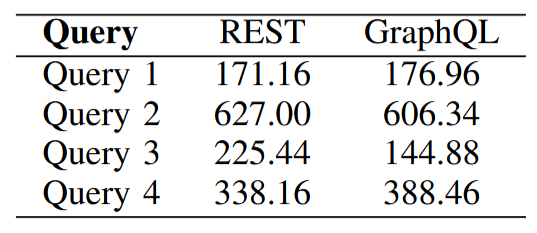
\includegraphics[scale=.5]{Illustrations/cangraphqlreplacerest.png}
\begin{BVerbatim}
Query 1: GET/user
Query 2: POST /repos/:owner/:repo/issues/:issue_number/comments
Query 3: GET/repos/:owner/:repo/issues/:issue_number
Query 4: GET/repos/:owner/:repo/stargazers
\end{BVerbatim}
	\caption{Latenz GraphQL vs. REST \citep{graphqlreplacerest}}
\end{figure}
\noindent
Die erste Abfrage (GET/user) zeigt, dass die Latenz zwischen REST und GraphQL sich nicht signifikant unterscheiden. REST benötigt für diese Anfrage 171,16 Millisekunde, während GraphQL mit 176,96 Millisekunden nur geringfügig langsamer ist. Dies lässt darauf schließen,dass bei einfachen Anfragen, die keine komplexe Datenstruktur beinhalten, sich die Ergebnisse nicht gravierend unterscheiden und als nahezu identisch bezeichnet werden können.
Die zweite Abfrage (POST /repos/:owner/:repo/issues/:issue\_number/comments), eine Schreiboperation, zeigt ein ähnliches Ergebnis. Hierbei ist GraphQL mit 606,34 Millisekunden leicht schneller als REST mit 627 Millisekunden. Da der Unterschied sehr gering ist, deutet dies daraufhin, dass Schreiboperationen in beiden Technologien ähnlich effizient verarbeitet werden.
Eine deutlich Differenz zeigt sich bei der dritten Abfrage (GET/repos/:owner/ :repo/issues/:issue\_number). REST benötigt hierfür 225,44 Millisekunden, während GraphQL mit nur 144,88 Millisekunden deutlich schneller ist. Dies verdeutlicht die Stärke von GraphQL bei komplexeren Datenanforderungen. Da GraphQL in der Lage ist, mehrere Datenpunkte in einem einzelnen Aufruf zu bündeln, kann es die Anzahl der API-Aufrufe reduzieren und so effizienter arbeiten.
Die vierte Abfrage (GET/repos/:owner/:repo/stargazers) zeigt ein gegensätzliches Bild. Hier ist REST mit 338,16 Millisekunden schneller als GraphQL, welches 388,46 Millisekunden benötigt. Die liegt daran, dass die Abfrage keine komplexe Aggregation von Daten erfordert und der Overhead von GraphQL die Performance negativ beeinflusst.
Somit kann man sagen, dass REST in einem Szenario besser abgeschnitten hat als GraphQL, GraphQL in einem anderen Szenario besser abschneidet als REST und beide Technologien in zwei Szenarien ähnlich abgeschnitten haben. 
\citep{graphqlreplacerest}
\newline
Andere Studien zeigen, dass GraphQL bei einfachen Abfragen, die nur einen Endpunkt nutzen, etwa 0,02-mal schneller als REST arbeitet. \citep{migrategraphql}
\newline
Bei komplexeren Anfragen, die vier Endpunkte umfassen und 1000 Ergebnistupel liefern, verarbeitet eine GraphQL-API die Daten bis zu 16-mal schneller als eine REST-API.\citep{analysegraphql}
\newline
Noch anspruchsvollere Anfragen, die fünf oder mehr Endpunkte nutzen, werden von GraphQL sogar bis zu 187-mal schneller bearbeitet.\citep{analysewebgraphql}
\newline
Bei steigender Komplexität stellt sich jedoch bei einer Menge von 100.000 Ergebnistupeln heraus, dass eine GraphQL API in diesem Fall 0.36 \citep{analysegraphql} bis 2,5 mal langsamer ist, als eine vergleichbare REST API \citep{restvsgraphql}.
%section ff1 (end)
\section{FF-2: Wie beeinflussen graph- und relationale Datenbanken die Latenz von REST- und GraphQL-APIs?} % (fold)
\label{sec:ff2}
Da APIs nur eine Schnittstelle zwischen einer Datenbank und der Anwendung darstellt, welche die Daten aus der Datenbank konsumieren möchte, ist die Latenz einer API zwingend von der Bearbeitungszeit einer Anfrage innerhalb der Datenbank abhängig. Hierbei nutzen verschiedene Datenbanktypen unterschiedlichste Methoden, um die angefragten Daten aus der Datenbank bereitzustellen. In dieser Arbeit wird ein besonderes Augenmerk auf die Verarbeitung anhand der relationalen Algebra, sowie der Graphentheorie gelegt. Diese Methoden bieten bei verschiedenen Anwendungsszenarien Vorteile, als auch Nachteile bei der Effizienten und Zeitsparenden Bearbeitung von Anfragen. Hierbei zeigt sich bei relationalen Datenbanken, dass diese bei steigender Anzahl an Daten, welche gespeichert werden zunehmend langsamere Performance bieten.
Wie in Abbildung 3.2 jedoch zusehen ist steigt die Menge der Daten, welche im Internet verarbeitet werden, seit 2010 bis heute stetig an und die Prognosen bis ins Jahr 2028 deuten auf einen deutlichen Trend zu erheblich mehr Daten an. Graphdatenbanken können mit solch einem Wachstum deutlich besser umgehen, da durch die Nutzung von Traversal-basierenden Anfragen, welche für diese  Art von Abfragen optimiert sind, die Menge die Menge der Daten innerhalb der Datenbank eine untergeordnete Rolle spielen. \citep{9677042} \citep{performancenosql}
\begin{figure}[H]
	\centering
	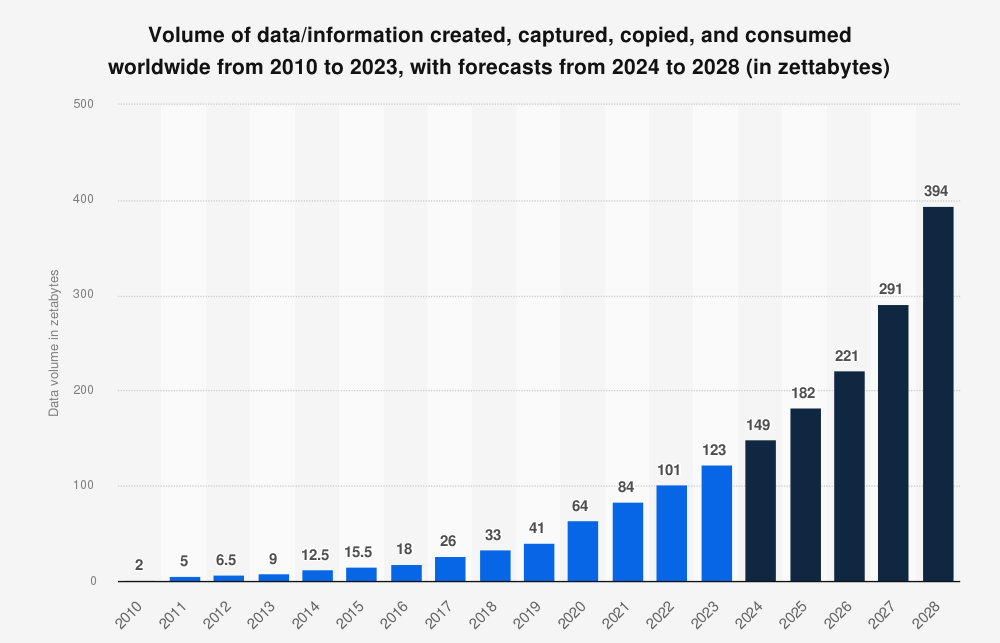
\includegraphics[scale=.4]{Illustrations/growthofdata.png}
	\caption{Datenmenge Weltweit \citep{statista}}
\end{figure}
\noindent
Ein weiterer Faktor, welcher die Performance einer Datenbank beeinflusst, ist die Verbundenheit, also die Relationen, der Daten. Abbildung 3.3 zeigt, wie sich die Verbundenheit der Daten im Verlauf verändert hat. Hierbei ist deutlich zu sehen, dass Daten stetig eine größere Verzweigung zueinander aufweisen. 

\noindent
Eine Graphdatenbank kann mit diesem hohen Grad an Verzweigung, durch die Verwendung der Graphentheorie und Traversierung performant umgehen.  Bei relationalen Datenbanken stellt diese hohe Grad der Relationen eine Performance Einbuße dar.  Da bei der Verbindung der Daten die Relationen zwischen der Tabellen durch Joins realisiert werden und diese aufwendig zu berechnen sind, steigt mit zunehmender Anzahl der Relationen auch die Zeit, welche die Datenbank benötigt um mithilfe der Schlüssel und mehrerer Tabellen die Beziehung zwischen den Dateneinträgen zu konstruieren. \citep{9677042} \citep{graphdb}
\begin{figure}[H]
	\centering
	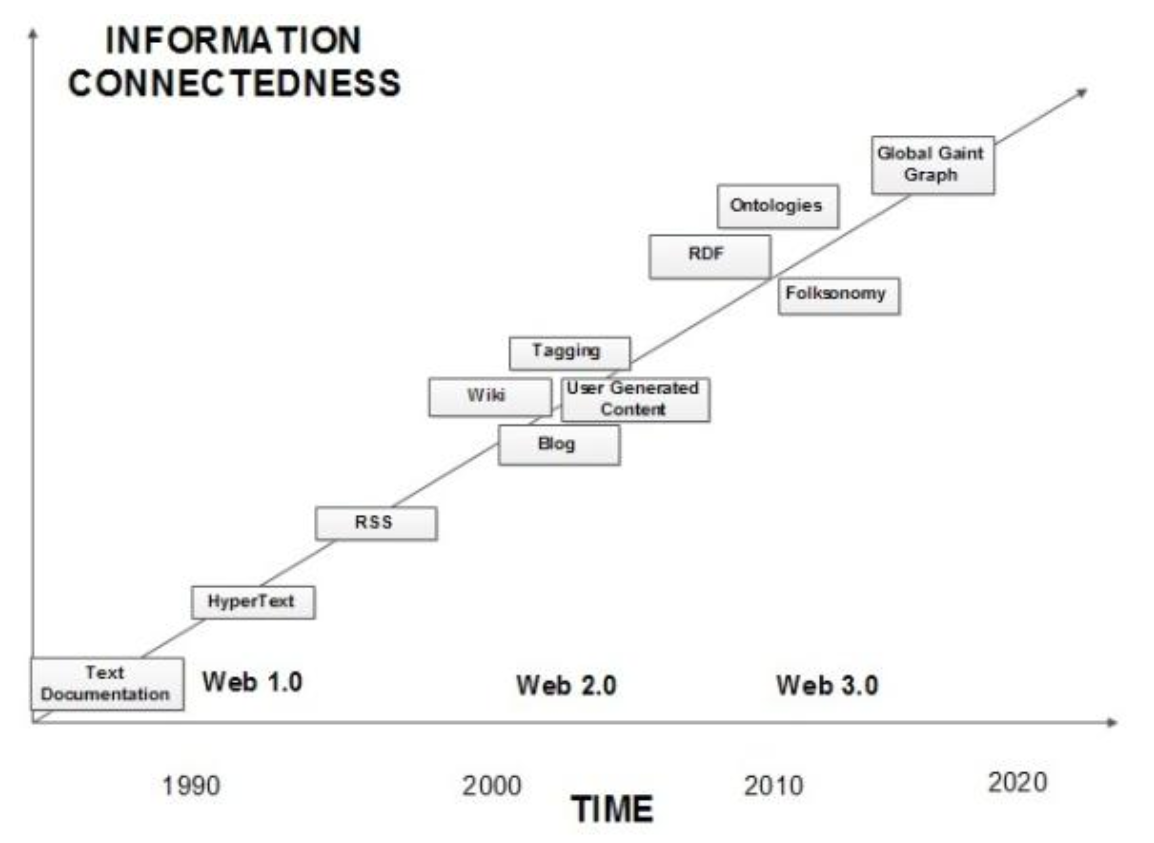
\includegraphics[scale=.45]{Illustrations/informationconnectedness.png}
	\caption{Informationsverbundenheit \citep{performancenosql}}
\end{figure}
\noindent
Die Universität von Mississippi führte ein Experiment durch, um die Latenzunterschiede zwischen einer relationalen MySQL-Datenbank und einer Graphdatenbank, konkret Neo4j, zu untersuchen. Dabei wurden sieben unterschiedliche Szenarien simuliert, deren Ergebnisse in den Abbildungen 3.4 und 3.5 dokumentiert sind. In der ersten Spalte der Tabelle wird die Konfiguration der Datenbank dargestellt. Hierbei gibt die Zahl die Anzahl der Nodes oder Tupel in der Datenbank an, gefolgt von einem Datentyp, der beschreibt, welche Art von Daten bei der Erstellung der Datenbank zufällig verwendet wurde.
Die Ergebnisse beider Datenbanken sind in Abbildung 3.4 zu sehen, wobei die Abfragen I1 und I2 unterschiedliche Szenarien repräsentieren. Die Abfrage I1 selektiert alle Nodes, deren Payload einem bestimmten Wert entspricht, während I2 die Nodes zählt, deren Payload kleiner ist als ein gegebener Wert. Beide Szenarien nutzen den Datentyp Integer um die Daten anzufordern. Aus den experimentellen Daten wird deutlich, dass die relationale MySQL-Datenbank im Vergleich zur Graphdatenbank Neo4j eine deutlich geringere Latenz in jedem gestestenen Fall aufweist.
 \citep{graphrelationaldb}
\begin{figure}[H]
	\centering
	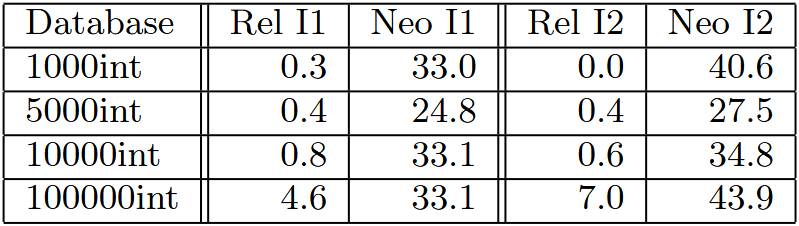
\includegraphics[scale=.5]{Illustrations/dbresultsint.png}
	\caption{Ergebnisse Abfragen durch int in Millisekunden \citep{graphrelationaldb}}
\end{figure}
\noindent
Abbildung 3.5 zeigt Abfragen, bei denen anhand eines Strings selektiert wurde. Die zweite Zeile gibt dabei an, welche Länge der String hatte, auf dessen Basis die Selektion vorgenommen wurde. Hierbei wird die Menge der Nodes gezählt, die den String enthalten. Die Ergebnisse zeigen ein deutlich anderes Bild im Vergleich zu den vorherigen Resultaten, bei denen mithilfe eines Integer selektiert wurde. Durch die Verwendung eines Strings kann die relationale Datenbank die Graphdatenbank lediglich im ersten Szenario übertreffen. In den komplexeren Fällen spielt die Graphdatenbank ihre Vorteile jedoch klar aus und ist bei anspruchsvolleren Anfragen in der Spitze um den Faktor 167 schneller.
 \citep{graphrelationaldb}
\begin{figure}[H]
	\centering
	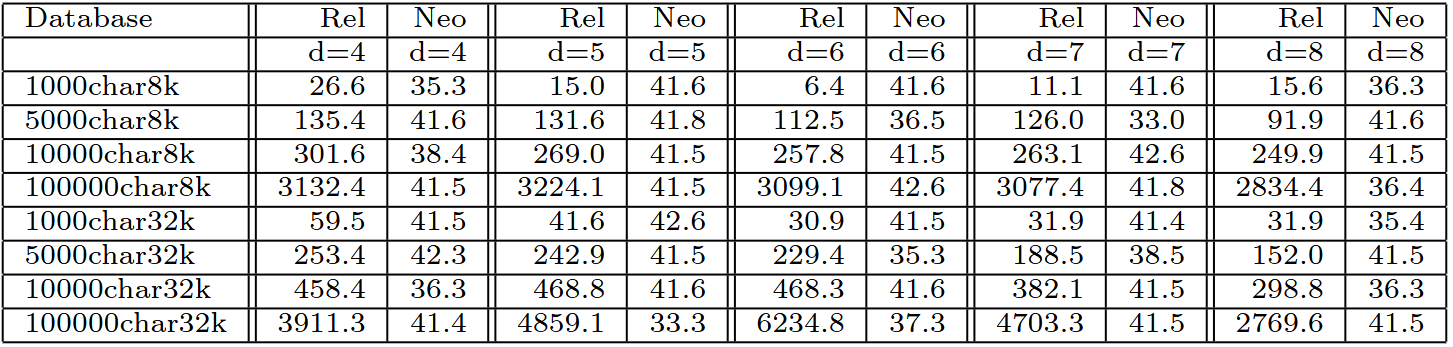
\includegraphics[scale=.425]{Illustrations/dbresultschar.png}
	\caption{Ergebnisse Abfragen durch char in Millisekunden \citep{graphrelationaldb}}
\end{figure}
\noindent
Zusammenfassend lässt sich feststellen, dass relationale Datenbanken bei der Selektion von Daten anhand eines Integer deutlich schnellere Ergebnisse liefern. Bei der Abfrage von Daten anhand eines Strings zeigt sich zunächst, dass relationale Datenbanken bei kleinen Datenmengen besser performen. Mit zunehmender Datenmenge wird jedoch die Graphdatenbank zunehmend effizienter und übertrifft schließlich die Performance der relationalen Datenbank deutlich.
%section ff2 (end)
% chapter analyse (end)